%%%%%%%%%%%%%%%%%%%%%%%%%%%%%%%%%%%%%%%%%
% Beamer Presentation
% LaTeX Template
% Version 1.0 (10/11/12)
%
% This template has been downloaded from:
% http://www.LaTeXTemplates.com
%
% License:
% CC BY-NC-SA 3.0 (http://creativecommons.org/licenses/by-nc-sa/3.0/)
%
%%%%%%%%%%%%%%%%%%%%%%%%%%%%%%%%%%%%%%%%%

%----------------------------------------------------------------------------------------
%	PACKAGES AND THEMES
%----------------------------------------------------------------------------------------

\documentclass{beamer}

\mode<presentation> {

% The Beamer class comes with a number of default slide themes
% which change the colors and layouts of slides. Below this is a list
% of all the themes, uncomment each in turn to see what they look like.

%\usetheme{default}
%\usetheme{AnnArbor}
%\usetheme{Antibes}
%\usetheme{Bergen}
%\usetheme{Berkeley}
%\usetheme{Berlin}
%\usetheme{Boadilla}
%\usetheme{CambridgeUS}
%\usetheme{Copenhagen}
%\usetheme{Darmstadt}
%\usetheme{Dresden}
%\usetheme{Frankfurt}
%\usetheme{Goettingen}
%\usetheme{Hannover}
%\usetheme{Ilmenau}
%\usetheme{JuanLesPins}
%\usetheme{Luebeck}
\usetheme{Madrid}
%\usetheme{Malmoe}
%\usetheme{Marburg}
%\usetheme{Montpellier}
%\usetheme{PaloAlto}
%\usetheme{Pittsburgh}
%\usetheme{Rochester}
%\usetheme{Singapore}
%\usetheme{Szeged}
%\usetheme{Warsaw}

% As well as themes, the Beamer class has a number of color themes
% for any slide theme. Uncomment each of these in turn to see how it
% changes the colors of your current slide theme.

%\usecolortheme{albatross}
%\usecolortheme{beaver}
%\usecolortheme{beetle}
%\usecolortheme{crane}
%\usecolortheme{dolphin}
%\usecolortheme{dove}
%\usecolortheme{fly}
%\usecolortheme{lily}
%\usecolortheme{orchid}
%\usecolortheme{rose}
%\usecolortheme{seagull}
%\usecolortheme{seahorse}
%\usecolortheme{whale}
%\usecolortheme{wolverine}

%\setbeamertemplate{footline} % To remove the footer line in all slides uncomment this line
%\setbeamertemplate{footline}[page number] % To replace the footer line in all slides with a simple slide count uncomment this line

%\setbeamertemplate{navigation symbols}{} % To remove the navigation symbols from the bottom of all slides uncomment this line
}

\usepackage{graphicx} % Allows including images
\usepackage{booktabs} % Allows the use of \toprule, \midrule and \bottomrule in tables

%----------------------------------------------------------------------------------------
%	TITLE PAGE
%----------------------------------------------------------------------------------------

\title[BBB]{BigBlueButton} % The short title appears at the bottom of every slide, the full title is only on the title page

\author{Amit} % Your name
\institute[Indian Institute of Technology] % Your institution as it will appear on the bottom of every slide, may be shorthand to save space
{
IITB \\ % Your institution for the title page
\medskip
\textit{shriamit1@gmal.com} % Your email address
}
\date{\today} % Date, can be changed to a custom date

\begin{document}

\begin{frame}
\titlepage  % Print the title page as the first slide
\end{frame}

\begin{frame}
\frametitle{Discussion Topic} % Table of contents slide, comment this block out to remove it
\tableofcontents % Throughout your presentation, if you choose to use \section{} and \subsection{} commands, these will automatically be printed on this slide as an overview of your presentation
\end{frame}

%----------------------------------------------------------------------------------------
%	PRESENTATION SLIDES
%----------------------------------------------------------------------------------------

%------------------------------------------------
\section{Progress} % Sections can be created in order to organize your presentation into discrete blocks, all sections and subsections are automatically printed in the table of contents as an overview of the talk
%------------------------------------------------

\subsection{Authentication Enabled} % A subsection can be created just before a set of slides with a common theme to further break down your presentation into chunks

\begin{frame}
\frametitle{Password Implementation}
\begin{itemize}

\item By default conference start with authentication.\pause
\item Authentication implemented by change dir in /var/www/bbb-default/index.html\pause
\item Change page is demo3.jsp 
\end{itemize}
\end{frame}
%new section added
\subsection{Conferencing Room development}
\begin{frame}
\frametitle{Conferencing features}
\begin{itemize}

\item audio/video/desktop share at client end.\pause
\item desktop share is enabled on client by jre.\pause
\item desktop share jar file is located inside /var/www/bigbluebutton/client
\end{itemize}
\end{frame}

%%new subsection 
\subsection{Scheduling}
\begin{frame}
\frametitle{Scheduling}
\begin{itemize}

\item Create meeting using create.jsp.\pause 
\item email pwd to users.\pause
\item dataSubmit.jsp,Meetingdetails.jsp pages are used.\pause
\item meeting info also send by sms.

\end{itemize}
\end{frame}


\subsection{Mobile conference}
\begin{frame}
\frametitle{Mobile Features}
\begin{itemize}
\item bbb-app is used to connect the meeting.\pause
\item salt authentication is need to added on server end.\pause
\item mobile\_conf.jsp page is use to add password.
\end{itemize}
\end{frame}
%------------------------------------------------
\section{New Development}
%------------------------------------------------
\subsection{Record Meeting}
\begin{frame}
\frametitle{Matterhorn}
\begin{itemize}

\item Configured Matterhorn on server with IP 10.107.91.88.\pause
\item It process the files send by bbb server. \pause
\item ffmpeg used to process the file.\pause
\item Caption can be added to the videos.\pause
\item Desktop share need to enable for record the meeting.
\end{itemize}
\end{frame}
%------------------------------------------------

\subsection{Technote}
\begin{frame}
\frametitle{Technote Features}
\begin{itemize}

\item Implemented on windows client.
\end{itemize}
\end{frame}
%------------------------------------------------

\subsection{Version 0.81}
\begin{frame}
\frametitle{BBB 0.81}
\begin{itemize}

\item Its developer version.\pause
\item Layout options as per meeting.\pause
\item Bandwidth monitor.\pause
\item Shortcut keys.\pause
\item New desktop share button.\pause
\item Color scheme is changed.\pause
\item Whiteboard is improved. 
\end{itemize}
\end{frame}

\subsection{Source Code}
\begin{frame}
\frametitle{Compilation}
\begin{itemize}
\item Source code is downloaded.\pause
\item Compilation of the code after making changes.\pause
\item Apache ANT java build up tool is used.\pause
\item bbb-conf tools are used.
\end{itemize}
\end{frame}

\section{Architecture}

\begin{frame}
\frametitle{Interaction of components}
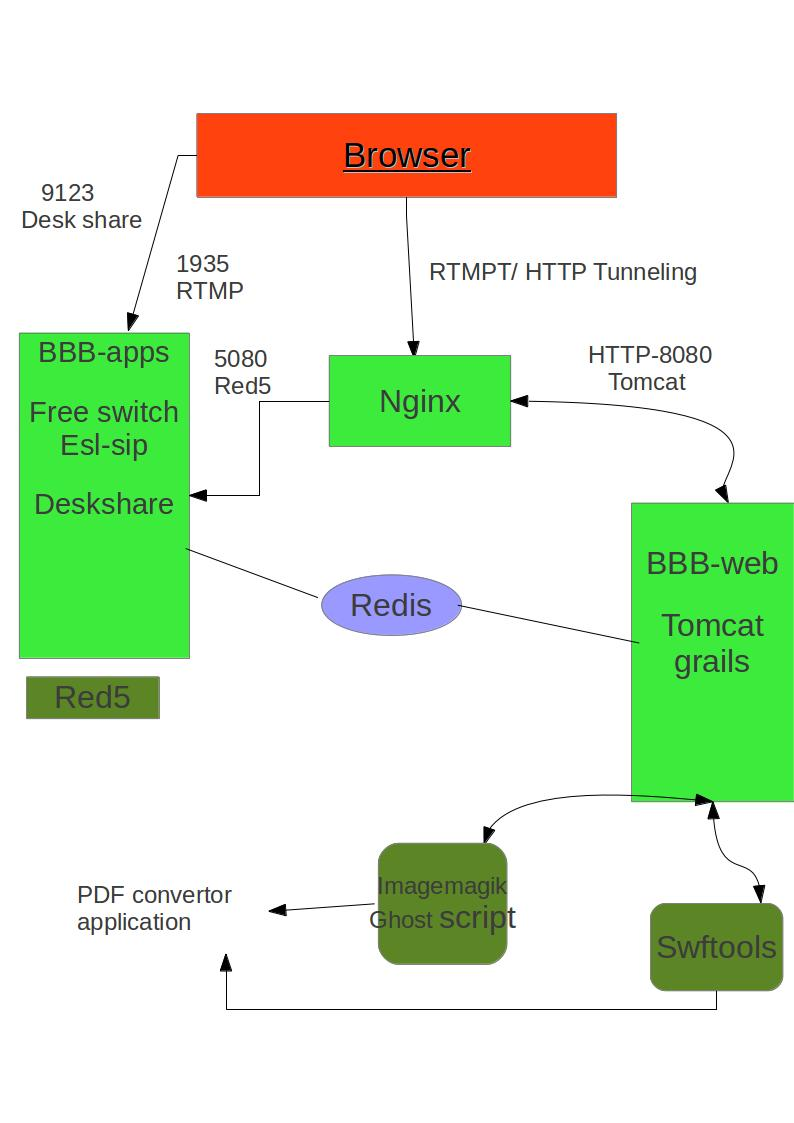
\includegraphics[width=90mm,height=90mm]{bbb.jpg}

\end{frame}
\end{document} 
